\documentclass[10pt,twocolumn,a4paper]{article}
\usepackage[a4paper,margin=.65in,columnsep=.25in]{geometry}
\usepackage[T1]{fontenc}\usepackage[utf8]{inputenc}\usepackage{mathptmx}
\usepackage{graphicx,amsmath,booktabs,hyperref}
\title{Bina.az Listing Price and Tier Prediction}
\author{MLE-AI-201 Final Project V3\\[2pt]\small PegaSold: Emiliya Abdulhalimova, Aygun Asvarova, Murad Bagirzade, Kanan Karimli}
\date{October 2026}
\begin{document}\maketitle
\begin{abstract}
We implement a NumPy decision tree for log-price regression and median-tier classification, and a NumPy Pegasos SVM with a random Fourier feature alternative. Of 100,775 raw rows, 57,543 remain after normalized advert-ID deduplication, Baku residential scope selection, and declared domain bounds. The training-only tier cut is 208,000 AZN. The scratch tree test RMSE is 0.239 in log-price space (147,356 AZN); scratch tree and Pegasos test F1 are 0.923 and 0.903. Asking prices are not verified transactions.
\end{abstract}
\section{Data and preprocessing}
The source contains Azerbaijani text fields, mixed missingness, repeat scrapes, and categories with different measurement units. The pipeline keeps Baku listings from the three residential categories. It normalizes numeric IDs from advert URLs and retains each ID's last dated scrape. Candidate reposts sharing coordinates, area, rooms, and price are reported but not deleted because the key does not establish that two ads describe one property. Fixed domain checks require price 10,000--5,000,000 AZN, area 10--2,000 m$^2$, unit price 200--20,000 AZN/m$^2$, plausible room counts, and valid stated floors. After splitting, a two-sided modified-z MAD fence is estimated from training `log(price)` only (cutoff 3.5) and applied only to training. All validation/test rows are retained, so the test metrics include outlier tails. The processed split is 40,033/8,632/8,632 (seed 42). Split allocation uses global-median price bins; the premium threshold is separately learned from the remaining training rows only.

The 80-column matrix contains 20 continuous/binary features and one-hot category/location columns. Train-only medians fill rooms/coordinates; train-only population means/stds scale continuous features. IDs, free text, views, `unit\_price`, and `total\_price` are excluded from model inputs. The raw file is never overwritten.
\begin{figure}[t]\centering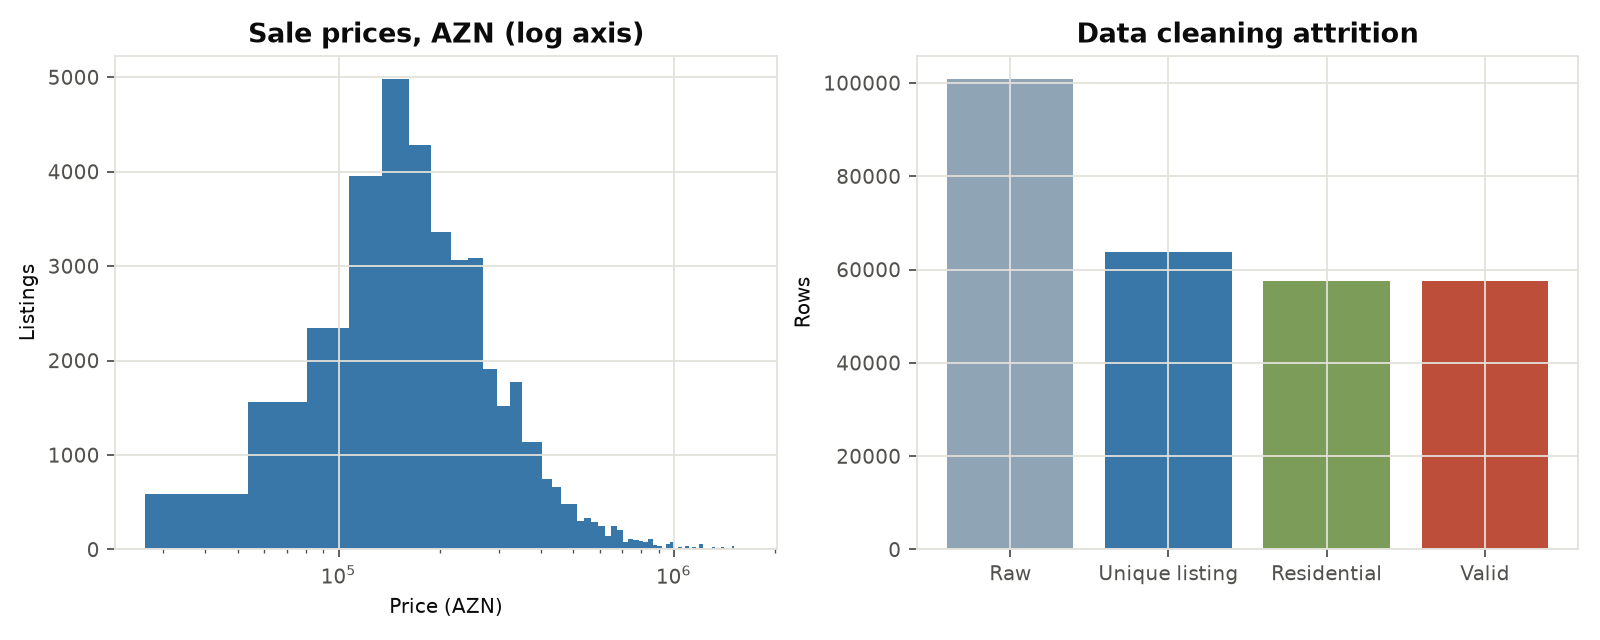
\includegraphics[width=\linewidth]{../reports/figures/data_and_prices.png}\caption{Row counts through cleaning and training price distribution.}\end{figure}
\section{Models and evaluation}
The NumPy tree tests numeric threshold midpoints. Gini/entropy use cumulative class counts; regression uses variance/MSE reduction via cumulative sums and squared sums. Leaves predict a majority class or target mean. Depth and minimum leaf settings are chosen from validation evidence.

Pegasos minimizes $J(w,b)=\frac{\lambda}{2}\|w\|^2+\frac{1}{n}\sum_i\max(0,1-y_i(w^Tx_i+b))$. It uses $\eta_t=1/(\lambda t)$, weight shrinkage, and hinge-loss subgradients. The intercept update is bounded by $\min(\eta_t,1)$ and is unregularized. The nonlinear option maps inputs to $\sqrt{2/D}\cos(xW+\phi)$ with 128 seeded random Fourier features. Library trees and SVMs are benchmark references; the course models remain project NumPy implementations.

We select model settings on validation, then report the held-out test once. Five-fold CV uses all 40,033 post-cleaning training rows and reports fold mean and standard deviation; each fold trains on four fifths and validates on one fifth. Regression CV also reports AZN-space MAE. Shared feature preprocessing was fitted before fold creation, so it is not fully nested CV. Validation and test data are not part of CV. Regression metrics are reported in both $\ln(\mathrm{AZN})$ and AZN. Classification reports accuracy, precision, recall, F1, ROC-AUC and confusion matrices.
\section{Held-out results}
\begin{table}[h]\centering\small\begin{tabular}{lrrr}\toprule Model & RMSE log & RMSE AZN & $R^2$ AZN\\\midrule
Scratch tree & 0.239 & 147,356 & 0.652\\
sklearn tree & 0.239 & 147,683 & 0.650\\\bottomrule\end{tabular}\caption{Held-out Task A results.}\end{table}
\begin{table}[h]\centering\small\begin{tabular}{lrrr}\toprule Model & Accuracy & F1 & ROC-AUC\\\midrule
Scratch tree & 0.922 & 0.923 & 0.958\\
sklearn tree & 0.922 & 0.923 & 0.959\\
Pegasos & 0.902 & 0.903 & 0.968\\\bottomrule\end{tabular}\caption{Held-out Task B results.}\end{table}
\begin{figure}[t]\centering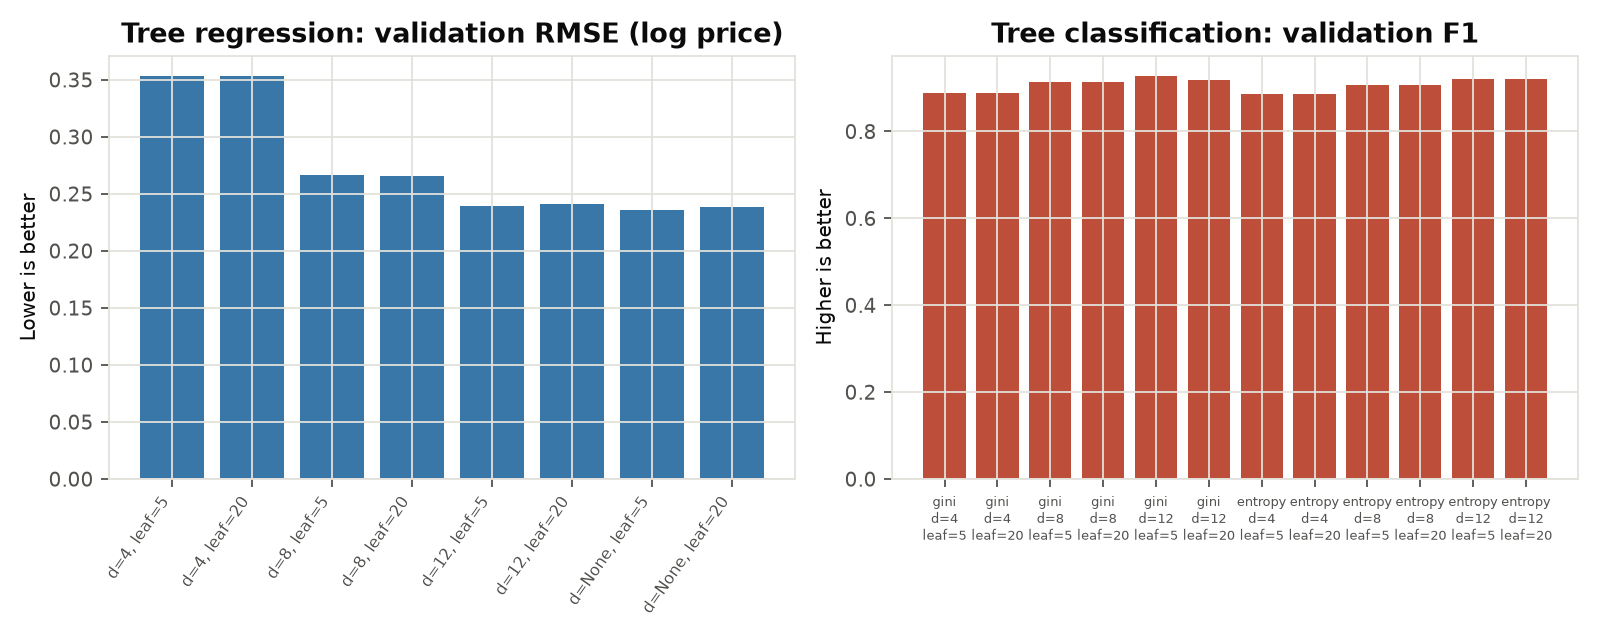
\includegraphics[width=\linewidth]{../reports/figures/tree_tuning.png}\caption{Validation-based tree sweeps.}\end{figure}
\begin{figure}[t]\centering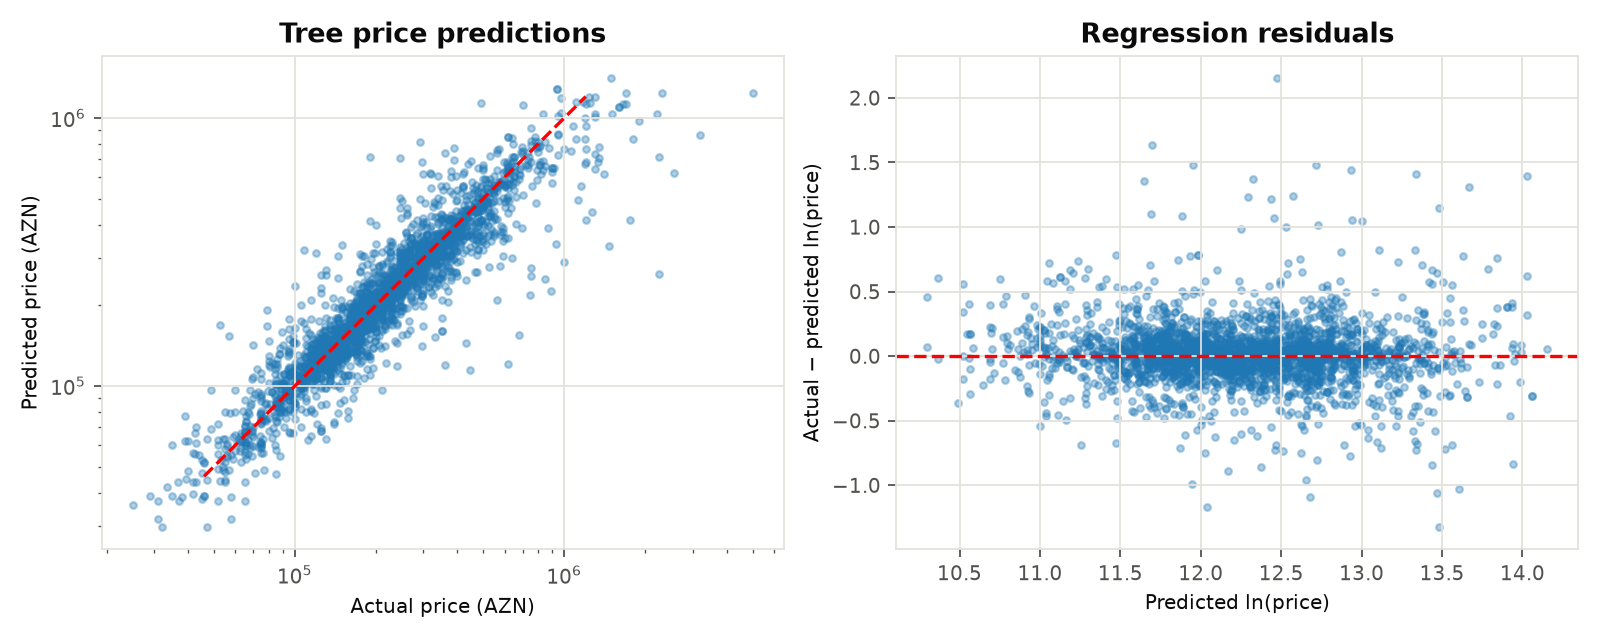
\includegraphics[width=\linewidth]{../reports/figures/regression_error_analysis.png}\caption{Predictions and residual analysis.}\end{figure}
\begin{figure}[t]\centering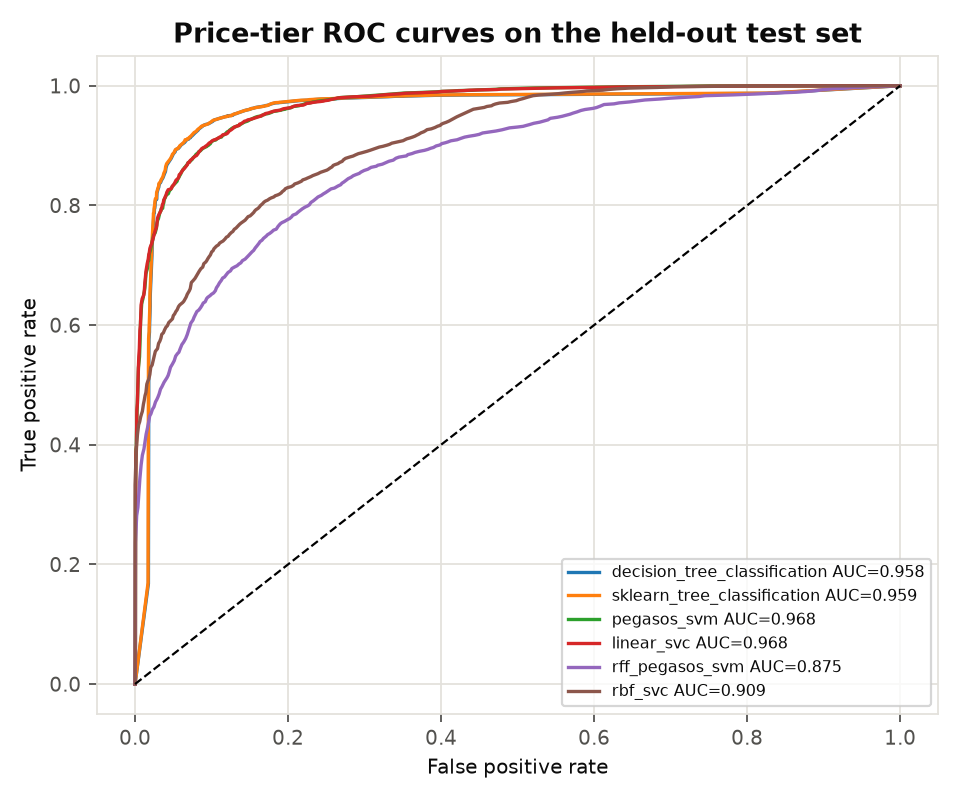
\includegraphics[width=\linewidth]{../reports/figures/roc_curves.png}\caption{ROC curves on held-out rows.}\end{figure}
\section{Limitations}
The target is advertised price rather than transaction price; the data are a 2024 scrape and do not describe today's market. Fixed value bounds were selected after full-source EDA. Ambiguous duplicate advertisements under different IDs may remain. CV shares preprocessing learned before folds. Impurity importance/correlation are descriptive rather than causal. Log-space prediction transformed with an exponential does not include a smearing correction for arithmetic conditional means.
\section*{AI-assistance disclosure}
AI assisted with coding suggestions, debugging, corrections, review, tests, visualizations, and documentation. The team is responsible for checking the final code and results. The decision tree and Pegasos algorithms are implemented in project NumPy code; scikit-learn supplies comparison models and standard utilities.
\end{document}
